\header{
    \section{Le Forban (version alternative)} \label{le-forban-alt}
    %
    
    \insertComment{Version de Michel Yaouank.}{}
}

\enluminure{4}{\href{https://www.youtube.com/watch?v=PKGcRHov0BU}{A}}{ moi} Forban que m'importe la gloire
\\Né fils de roi et de prostituée
\\Sur des cadavres j'ai chanté la victoire
\\Et dans un crâne j'ai bu la liberté
\\Vierge craintive, toi, ma captive
\\Tes vertus vont expirer dans mes bras
\\Ce soir je vais dévorer tes appâts
\\Encore brûlant d'une autre amante
\\Ce soir je vais dévorer tes appâts
\\\\\textbf{Refrain :}
\\Vin qui pétille, femme gentille
\\Sous tes baisers brûlant d'amour, oui d'amour
\\Plaisir bataille vive la canaille
\\Je bois, je chante et je tue tour à tour.
\\\\Pendu au mât d'une barque étrangère
\\Mon corps un jour servira d'étendard
\\Et tout mon sang rougira la galère
\\Aujourd'hui fête et demain le hasard
\\Allons esclaves, debout mes braves
\\Buvons l'ivresse et l'orgie à grands flots
\\Aujourd'hui fête , demain peut être
\\Mon corps ira s'engloutir dans les flots
\\\\Etant Forban je vis dans ma cabine
\\En méprisant les lois , même la mort
\\Ne vivant que de meurtre et de rapine
\\Je bois mon vin dans une coupe d'or
\\Vivre d'orgie est ma seule espérance
\\Le seul bonheur que j'ai su conquérir
\\Car sur les flots j'ai bercé mon enfance
\\Et sur les flots un Forban doit mourir.
\breakpage
Si par hasard par un coup de fortune
\\Je capturais l'or d'un beau galion
\\Riche à pouvoir décrocher la lune
\\Je m'en irai vers d'autres horizons
\\Là vénéré tout comme un gentilhomme
\\Moi qui ne fut qu'un Forban qu'un bandit
\\Là je pourrais peut être tout comme
\\Un roi dormir dans un bon lit.
\\
\begin{center}
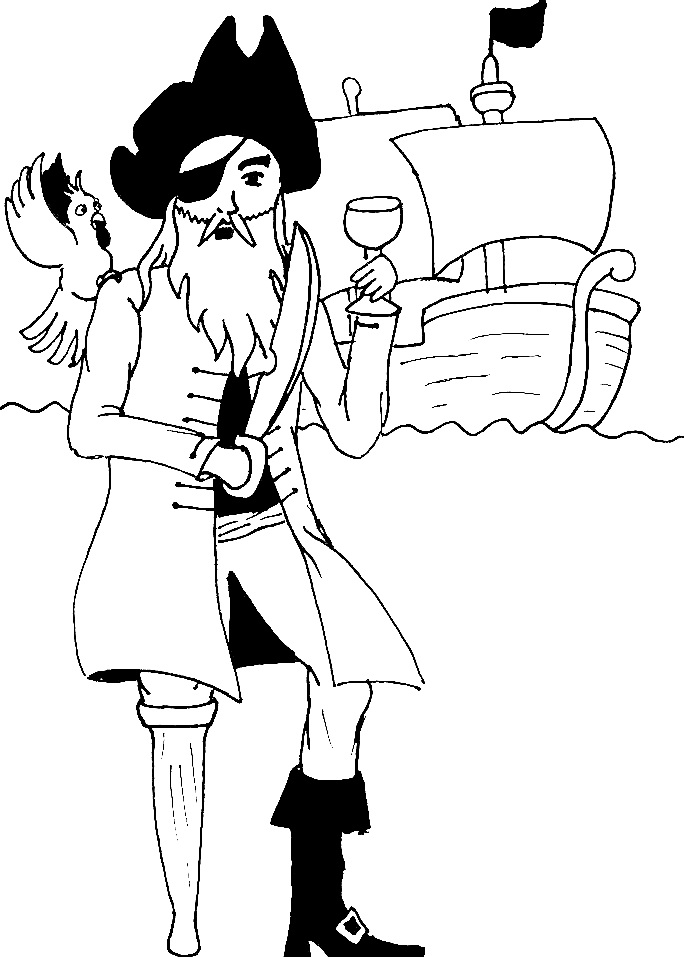
\includegraphics[width=0.8\textwidth]{images/chant_corsaire.jpg}
\end{center}

\breakpage